\begin{savequote}[75mm]
This is a quote.
\qauthor{Author}
\end{savequote}

\chapter{Introduction}
\section{Motivation}
\subsubsection{Questions}
 Can quantiative forecasting play a central role in enhancing our understanding of global emissions? Will it allow us to make strategic decisions when decarbonizing? Can we build a more sustainable future with a targeted approach that uses data to identify potential for improvement? What other data do we need to increase our prediction accuracy and understend the impact of business strategies on decarbonization? Can we predict future decarbonization rates and, if so, what is the best way to do it? \\ 
 \subsubsection{Why is this important? and the interesection of academic and business interest}
 \noindent Those are only a few of the very important and interesting questions that drew me to research decarbonization and to focus on the role of corporate emission-level data in the process. I believe that research in this area is crucial to advance our ability to build a more sustainable future. Furthermore, the answers to these questions can help us make better decisions and build a more sustainable future while also creating value for businesses. Additionally, the call for more data in decarbonization comes not only from the academic world but also from the fact that many business opportunities arise from the climate transition that inevitably requrie good and valid information to determine which companies and sectors are winners and loosers, which are the champions in the decarbonization process, which are the laggards, and which are the companies that are greenwashing. I believe that studying specifically corporate emissions and forecasting decarbonization rates as I am doing in this thesis can be useful to three key stakeholders: 
 \subsubsection{The key stakeholders}
 \begin{enumerate}
    \item \textbf{Investors} who are increasingly interested in understanding the climate risk of their portfolios and in identifying the companies that are best positioned to succeed in the transition to a low-carbon economy. For examples, companies such as BlackRock [insert quotation here] are enhancing their sustainable investing strategies and offering more sustainable investment products to their clients.
    \item \textbf{Companies} who are increasingly interested in understanding their climate risk and in identifying the best strategies to reduce their emissions and to succeed in the transition to a low-carbon economy. Additionally, companies might be interested in benchmarking against their peers in the sector to understand how they are performing relative to their competitors and to identify the best practices. 
    \item \textbf{Policy makers} who are increasingly interested in understanding the climate risk of their countries and in identifying the best strategies to reduce their emissions and to succeed in the transition to a low-carbon economy. A sector and company level analysis can be useful in determining optimal targets for new policies, identifying the best practices, and understanding the impact of new policies on the sector and on the economy.
\end{enumerate}

\subsubsection{Connection between computer science and decarbonization}
\noindent Finally, I believe that the use of data and modeling techniques  can help us build a more sustainable future in a practical, nonpolitical, and unbias way. Estimating emissions is an amazing example of how Computer Sicence and Statistical models can help us achieve real impact driving strategic decisions. I argue furthermore that it is only through a quantitative driven approach that we can dimistify the climate debate and make progress in the climate transition. I am confident that work in the modeling decarbonization has an incredible potential to create value for business and society and especially with increasing data availability and computational power, the time is ripe to make progress in this area. As I will explain in the next sections, this thesis is only possible thanks to incresased data availablity and to the willingness of corporates to disclose their emissions.


\subsection{Emission Scopes}
The thesis will assume familiarity with the concept of Scopes 1, 2, and 3 emissions which I am going to explain in this section. In carbon-accounting and emissions reporting, it is very important to distinguish between three types of emissions: Scope 1, Scope 2, and Scope 3 emissions. Each category represents a different level of emissions associated with an organization's activities. 

\begin{itemize}
    \item \textbf{Scope 1} emissions are direct emissions from owned or controlled sources. This includes emissions from company vehicles, and emissions from chemical processes or combustion in owned or controlled boilers, furnaces, etc.
    \item \textbf{Scope 2} emissions are indirect emissions from the generation of purchased electricity, steam, heating, and cooling consumed by the reporting company. These emissions occur at the facility where the energy is generated, not at the point of consumption.
    \item \textbf{Scope 3} emissions are all indirect emissions (not included in Scope 2) that occur in the value chain of the reporting company. This includes both upstream and downstream emissions, encompassing a wide range of activities such as the extraction and production of purchased materials, transportation of purchased fuels, and use of sold products and services.
\end{itemize}

\noindent Understanding these scopes is critical for organizations aiming to fully assess and manage their carbon footprint.

\newpage
\begin{figure}[h]
    \centering
    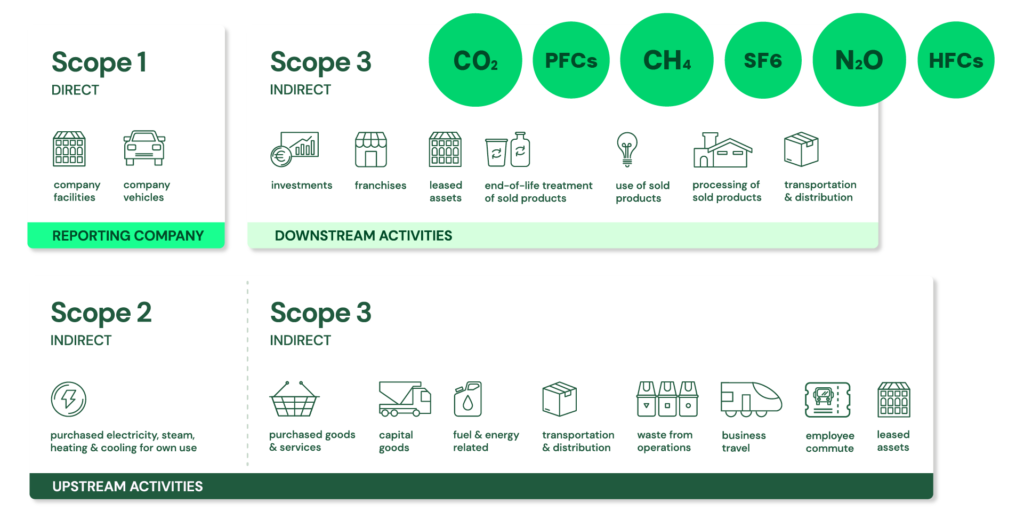
\includegraphics[width=0.8\textwidth]{figures/emission_scopes.png}
    \caption{Caption of Scopes 1, 2, and 3 Emissions. Adapted from \cite{Bernoville2022Scopes}.}
    \label{fig:my_label}
\end{figure}


\subsection{A business oriented framework to justify decarbonization}
\noindent The Paris Agreement sets forth ambitious objectives to combat climate change, aiming to cap the increase in global temperatures to 2°C, with an aspirational target of 1.5°C, above pre-industrial levels. This is to be achieved through a series of significant measures, including reaching net-zero greenhouse gas emissions by 2085 and a reduction of these emissions by 10\% by 2030 \cite{Sanderson2016What}. These goals require substantial transformations in global economic structures, especially in the realms of energy consumption and the development of renewable energy sources. For instance, in the United States, attaining deep decarbonization necessitates a national overhaul in the way energy is produced and used, with implications for urban planning and land management \cite{Hsu2022Planning}. Similarly, in the European Union, deep decarbonization could be pursued via either a demand-driven system or a centralized approach to manage carbon emissions. However, achieving more ambitious targets will require a broader mix of technologies and greater intersectoral synergy \cite{Korkmaz2020A}.

\noindent Numerous policy instruments, particularly carbon taxation, are progressively being implemented in major developed economies. Some experts advocate for a global carbon tax as a potent mechanism to expedite decarbonization in the energy sector. However, this approach encounters several hurdles, including substantial capital investment needs, competition between different sectors, varying environmental policies across regions, and the challenge of securing public acceptance for changes in energy consumption habits \cite{Papadis2020Challenges}.


\noindent In my opinion, regardless of the specific outcomes of a global carbon tax, the transition to a low-carbon economy is inevitable and will have a profound impact on the business world. This is because, despite the decrease in 2020 due to the COVID-19 pandemic, global energy-related CO 2 emissions remained at 31.5 Gt, contributing to CO2 reaching its highest ever average annual concentration in the atmo-sphere of 412.5 parts per million in 2020 – roughly 50\% higher than when the industrial revolution began. Global energy-related CO 2 emissions are expected to rebound and continue increasing, as demand for coal, oil, and gas recovers along with the economy \cite{BHATT2023100095}. It seems like carbon emissions are arguably the greatest negative externality that is currently affecting global markets, we don't yet have a single global policy to regulate emissions, that is not game theory optimal for a country to commit to lowering emissions before others, but chances are that if the decabonization strategy is not implemented, the world will face a climate crisis that will have a profound impact on the economy. Interestingly, the more we wait to implement a decarbonization strategy, the more likely it will be that the transition will need to be more abrupt, and in this case firms that are not prepared will face significant risks, while firms that are prepared will have a competitive advantage. As Professor Serafeim argues, such transition should not be seen as an inefficiency, but rather as a demand for innovation and a source of new business opportunities \cite{purpose+profit}. Indeed, by transitioning to a low-carbon economy, companies can create value for their shareholders, employees, and society at large. Therefore, if a company is to succeed in a modern business landscape, it must do so by alignign its profit strategy with a concrete purpose strategy, which includes a commitment to lowering carbon emissions. When it comes to sustainability, the transition will require significant changes in the way companies operate, and it will create both risks and opportunities \cite{purpose+profit}. For instance, companies that are able to reduce their emissions will be better positioned to succeed in the transition, while companies that are unable to do so will face significant risks. The transition will also create opportunities for new business models and technologies, and it will require companies to adapt to new regulations and policies. In this context, it is crucial for companies to understand their climate risk and to identify the best strategies to reduce their emissions and to succeed in the transition to a low-carbon economy. This is where the role of data and modeling techniques becomes crucial. Not only can these techniques help companies understand their climate risk, but they can also help companies identify the best strategies to reduce their emissions and to succeed in the transition to a low-carbon economy. Under this framework, it is therefore not surprising to see that companies are increasingly interested in understanding their climate risk and in identifying the best strategies to reduce their emissions and to succeed in the transition to a low-carbon economy and are increasingly more willing to disclose them.

\section{Carbon Disclosure Project Data}
\begin{figure}[h]
    \centering
    
\includegraphics[width=0.8\textwidth]{figures/cdp_logo.png}
    \caption{Carbon Disclosure Project Logo. Adapted from \cite{CDPMain2024}.}
    \label{fig:my_label}
\end{figure}

The primary data source for this thesis is the Carbon Disclosure Project (CDP) Climate Change Questionnaire \cite{CDP2024}, which was kindly provided to me by the Climate and Sustainability Impact Lab from the Digital Design Institute at the Harvard Business School \cite{HarvardD3Lab2024}. The Carbon Disclosure Project is a not-for-profit charity that runs the global disclosure system for investors, companies, cities, states and regions to manage their environmental impacts \cite{CDPMain2024}. The importance of the CDP is widely recognized by the business and the academic communities. As Ban Ki Moon, former Secretary General of the United Nations, states ``The work of CDP is crucial to the success of global business in the 21st century... helping persuade companies throughout the world to measure, manage, disclose and ultimately reduce their greenhouse gas emissions. No other organization is gathering this type of corporate climate change data and providing it to the marketplace'' \cite{CDPMain2024}. The Carbon Disclosure Project Sustainability Questionnaire uses the Greenhouse Gas (GHG) Protocol as a reporting model for carbon-related data \cite{Andrew2011Accounting}. It is one of the largest datasets of self-reported GHG emissions and collects a wide range of information on climate change-related topics. The questionnaire provides a globally consistent disclosure standard for GHG emissions and information on a firm’s activities to reduce GHG emissions. The CDP is backed by a large number of institutional investors, including banks, insurance companies, asset management companies, and pension funds holding US\$100 trillion in assets (i.e., CDP signatories), which act as ``norm entrepreneurs'' \cite{OTT201714}. Currently more than 23,000 companies disclose their emission data through the survey, representing two thirds of global market capitalization \cite{CDPMain2024}. 

\subsubsection{Motivations Behind Corporate Disclosure to the CDP}
The Carbon Disclosure Project (CDP) questionnaire has not only gained increasing popularity among companies but has also become a pivotal tool for investors and other stakeholders in evaluating corporate climate risks. It plays a crucial role in identifying effective strategies for emission reduction and in navigating the transition towards a low-carbon economy. The growth in the completion and publication rates of the CDP questionnaire reflects its importance, with institutional investors exerting a notable influence on climate change disclosure through corporate communication channels \cite{Cotter2012Institutional}. Consequently, the annual increase in the number of companies engaging in disclosure highlights a substantial data pool, invaluable for analyzing the decarbonization process and projecting future emission trends. The rationale for companies to disclose varies, encompassing regulatory compliance, investor expectation alignment, reputation enhancement, peer benchmarking, emission reduction opportunity identification, and risk assessment. Furthermore, disclosing to CDP entails two independent steps: the first involves the completion of the questionnaire, while the second involves the publication of the response. The latter step is particularly significant, as it demonstrates a company’s commitment to transparency and accountability, thereby enhancing its reputation and credibility \cite{Cotter2012Institutional}.

\subsection{Current Metrics and Limitations}
The CDP survey assigns a score that ranks the performance of companies when decarbonizing. For reference, 48\% of S\&P companies scored high-performance band B ratings and above in their Carbon Disclosure Project (CDP) reports in 2014 \cite{Upadhyay2022Improving}. When assiging a score, CDP assesses the level of detail and comprehensiveness in a response, as well as the company’s awareness of environmental issues, its management methods and progress towards environmental stewardship \cite{CDP2022ScoringPDF}. Additionally, specifically for climate-change scores, to recieve an A-level grade a copmany must verify at least 70\% of Scope 1, Scope 2 and Scope 3 emissions with a CDP-approved verification standard. Among other criteria, to score an A on Climate Change, companies must have robust governance and oversight of climate issues, rigorous risk management processes, verified scope 1 and 2 emissions and be reducing emissions across their value chain. Most Climate Change A List companies as of 2022 have well established emissions targets that have been approved by the SBTi, and evidence of targets which cover their scope 3 emissions \cite{CDP2022ScoringPDF}. 


\begin{figure}[h]
    \centering
    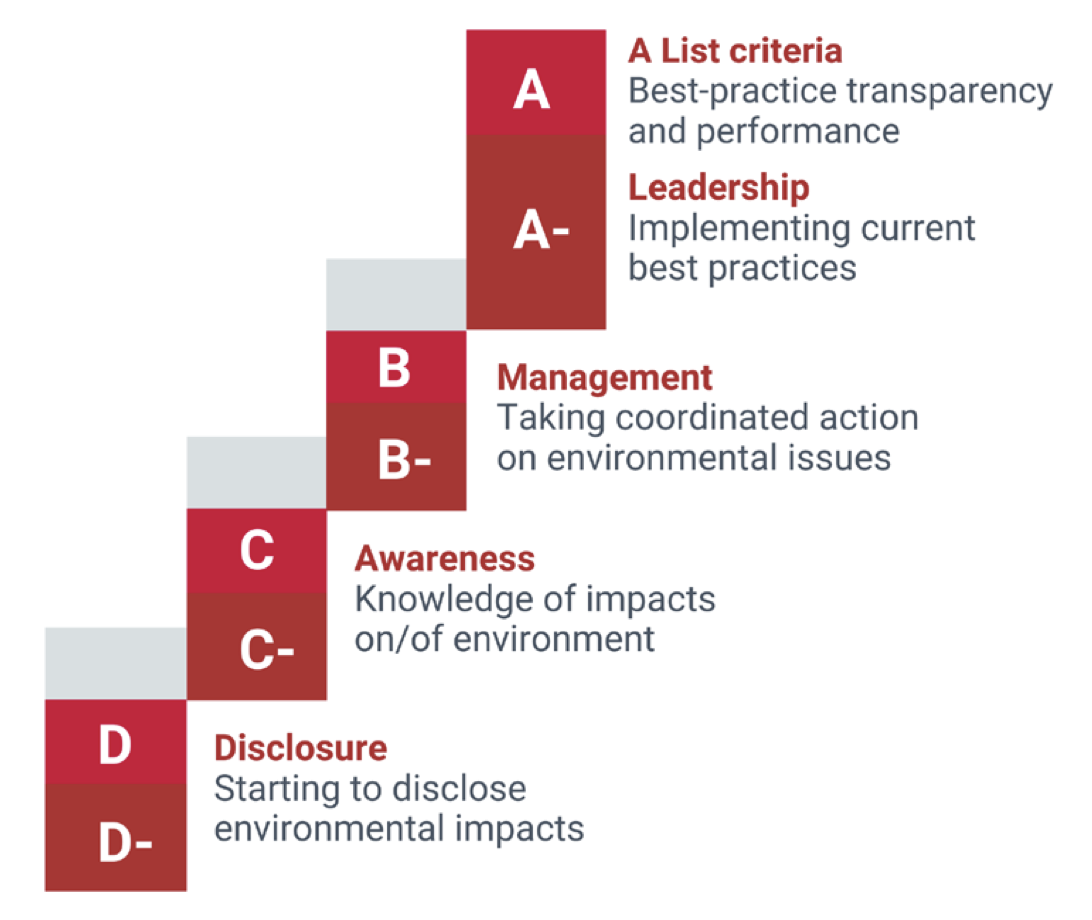
\includegraphics[width=0.8\textwidth]{figures/cdp_scoring.png}
    \caption{Caption of CDP Scoring Grades. Adapted from \cite{CDP2022ScoringPDF}.}
    \label{fig:my_label}
\end{figure}


\noindent While the CDP score is a valuable and widely recognized metric, it has several limitations. First, the CDP score is assigned based on adherance to best-practices and does not provide a future outlook on the company-specific ability to reduce emissions. It signals that the company is currently adhearing to best practices, but there is no immediate way to know by how much will the company be able to reduce its emissions in the future. Second, the CDP score is based on self-reported data, which can be subject to biases and errors. Third, the score does not provide an estimate of the company's future emissions, which is crucial for investors and policy makers. Thus, the score can be useful as a first metric and this leaves the door open for more sophisticated models to be developed which is the main goal of this thesis, in particular when it comes to forecasting next-year emissions and whether a company will perform better or worse in the future compared to its peers.
